\documentclass{beamer}\usepackage[]{graphicx}\usepackage[]{color}
%% maxwidth is the original width if it is less than linewidth
%% otherwise use linewidth (to make sure the graphics do not exceed the margin)
\makeatletter
\def\maxwidth{ %
  \ifdim\Gin@nat@width>\linewidth
    \linewidth
  \else
    \Gin@nat@width
  \fi
}
\makeatother

\definecolor{fgcolor}{rgb}{0.345, 0.345, 0.345}
\newcommand{\hlnum}[1]{\textcolor[rgb]{0.686,0.059,0.569}{#1}}%
\newcommand{\hlstr}[1]{\textcolor[rgb]{0.192,0.494,0.8}{#1}}%
\newcommand{\hlcom}[1]{\textcolor[rgb]{0.678,0.584,0.686}{\textit{#1}}}%
\newcommand{\hlopt}[1]{\textcolor[rgb]{0,0,0}{#1}}%
\newcommand{\hlstd}[1]{\textcolor[rgb]{0.345,0.345,0.345}{#1}}%
\newcommand{\hlkwa}[1]{\textcolor[rgb]{0.161,0.373,0.58}{\textbf{#1}}}%
\newcommand{\hlkwb}[1]{\textcolor[rgb]{0.69,0.353,0.396}{#1}}%
\newcommand{\hlkwc}[1]{\textcolor[rgb]{0.333,0.667,0.333}{#1}}%
\newcommand{\hlkwd}[1]{\textcolor[rgb]{0.737,0.353,0.396}{\textbf{#1}}}%

\usepackage{framed}
\makeatletter
\newenvironment{kframe}{%
 \def\at@end@of@kframe{}%
 \ifinner\ifhmode%
  \def\at@end@of@kframe{\end{minipage}}%
  \begin{minipage}{\columnwidth}%
 \fi\fi%
 \def\FrameCommand##1{\hskip\@totalleftmargin \hskip-\fboxsep
 \colorbox{shadecolor}{##1}\hskip-\fboxsep
     % There is no \\@totalrightmargin, so:
     \hskip-\linewidth \hskip-\@totalleftmargin \hskip\columnwidth}%
 \MakeFramed {\advance\hsize-\width
   \@totalleftmargin\z@ \linewidth\hsize
   \@setminipage}}%
 {\par\unskip\endMakeFramed%
 \at@end@of@kframe}
\makeatother

\definecolor{shadecolor}{rgb}{.97, .97, .97}
\definecolor{messagecolor}{rgb}{0, 0, 0}
\definecolor{warningcolor}{rgb}{1, 0, 1}
\definecolor{errorcolor}{rgb}{1, 0, 0}
\newenvironment{knitrout}{}{} % an empty environment to be redefined in TeX

\usepackage{alltt}
\usetheme{Warsaw}

\usepackage{polski}
\usepackage[utf8]{inputenc}
\setbeamerfont{caption}{size=\scriptsize}

\title{Wprowadzenie do Apache Spark}
\author{Justyna Jankowiak}
\institute{Koło Naukowe Data Science, MiNI}
\date{19.04.2016}
\IfFileExists{upquote.sty}{\usepackage{upquote}}{}
\begin{document}

\frame{\titlepage}

\begin{frame}
\frametitle{Co to jest Apache Spark?}

\begin{columns}
  \begin{column}{0.5\textwidth}
    \begin{itemize}
    \item Jest to szybki silnik do~przetwarzania dużych danych.
    \item Główną zaletą Sparka jest możliwość wykonywania obliczeń w pamięci, co~przyspiesza działanie aplikacji.
  \end{itemize}
  
  \end{column}
  \begin{column}{0.5\textwidth}  %%<--- here
    \begin{center}
      
\includegraphics[width=\textwidth]{spark_logo.png}
     \end{center}
  \end{column}
\end{columns}
\end{frame}

\begin{frame}
\frametitle{Historia rozwoju Sparka}
\begin{itemize}
\item \textbf{2009} - opracowanie oprogramowania na Uniwersytecie Kalifornijskim w Berkeley
\item \textbf{2010} - opublikowanie Sparka jako wolne oprogramowanie zgodnie z licencją BSD (Berkeley Software Distribution License)
\item \textbf{2013} - przekazanie Sparka do fundacji Apache Software
\item \textbf{od 2014} - Spark jest jednym z czołowych projektów Apache
\end{itemize}

\begin{columns}
  \begin{column}{0.5\textwidth}  %%<--- here
    \begin{center}
      
\includegraphics[width=\textwidth]{uni_logo.jpg}
     \end{center}
  \end{column}
  \begin{column}{0.5\textwidth}  %%<--- here
    \begin{center}
      
\includegraphics[width=\textwidth]{apache_logo.png}
     \end{center}
  \end{column}
\end{columns}
\end{frame}

\begin{frame}
\frametitle{Cechy Sparka}
\begin{itemize}
\item \textbf{Szybkość} - działa do 100 razy szybciej niż MapReduce z~wykorzystaniem pamięci operacyjnej i do 10 razy szybciej z~wykorzystaniem operacji dyskowych 
  \begin{figure}
  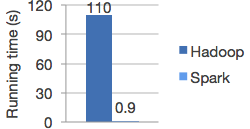
\includegraphics[width=0.3\textwidth]{logistic-regression.png}
  \vspace{-10pt}
  \caption{Źródło: http://spark.apache.org/}
  \end{figure}
\item \textbf{Łatwy w użyciu} - możliwość budowania aplikacji z~wykorzystaniem języków Java, Scala, Python lub R
\item \textbf{Zaawansowana analityka} - nie tylko operacje `map-reduce` ale również SQL, strumienie danych, machine learning oraz~algorytmy grafowe
\end{itemize}
\end{frame}

\begin{frame}
\frametitle{RDD}
\textbf{Resilient Distributed Datasets} (leniwe kolekcje rozproszone :)) to~podstawowa struktura danych w Sparku. 
\begin{itemize}
\item Możliwość wykonywania równoległych operacji
\item Sposoby tworzenia RDD
\begin{itemize}
\item operacja \textit{parallelize} na "zwykłych" obiektach (np. liście) 
\item odwołanie do zewnętrznych źródeł danych (np. lokalny system plików lub HDFS)
\end{itemize}
\item Wykonujemy na nich dwie operacje
\begin{itemize}
\item transformacje (np. \textit{map}, \textit{filter})
\item akcje (np. \textit{collect}, \textit{reduce})
\end{itemize}
Wszystkie transforacje są leniwe, tzn. nie są wykonywane dopóki nie jest to konieczne. Wykonywane są dopiero, gdy następujące po nich akcje wymagają zwrócenia wyniku. 
\end{itemize}
\end{frame}

\begin{frame}
\frametitle{Rozszerzenia Spark Core}
\begin{figure}
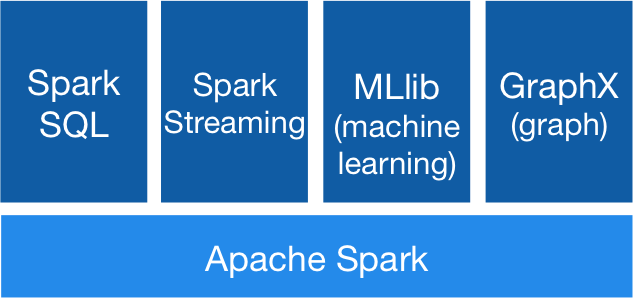
\includegraphics[width=\textwidth]{spark_components.png}
  \vspace{-10pt}
  \caption{Źródło: http://spark.apache.org/}
\end{figure}
\end{frame}

\begin{frame}
\frametitle{Co dalej?}
Zachęcam do uczestnictwa w bezpłatnych kursach na platformie e-learningowej edX:

https://www.edx.org/xseries/data-science-engineering-spark

\end{frame}

\end{document}
